\documentclass{article}

\usepackage{geometry}
\usepackage{makecell}
\usepackage{array}
\usepackage{multicol}
\usepackage{setspace}
\usepackage{changepage}
\usepackage{cprotect}
\usepackage{booktabs}
\usepackage{graphicx}
\usepackage{float}
\newcolumntype{?}{!{\vrule width 1pt}}
\newcommand{\paragraphlb}[1]{\paragraph{#1}\mbox{}\\}
\renewcommand\theadalign{tl}
\setstretch{1.10}
\setlength{\parindent}{0pt}

\geometry{top=12mm, left=1cm, right=2cm}
\title{\vspace{-1cm}Netzwerktechnologien Aufgabenblatt 5}
\author{Andreas Hofer}

\begin{document}
	\maketitle
	\section{Inter-Domain Routing}
	\begin{center}
		\begin{tabular}{| c | c | c | c | c |}
			\toprule
			Subnetzadresse & Subnetzmaske & Nächster Hop & Schnittstelle & Hop Count \\ \midrule
			192.168.1.0 & 255.255.255.255 & 10.1.1.1 & 10.1.1.2 & 2 \\
			192.168.2.0 & 255.255.255.255 & 192.168.2.1 & 192.168.2.1 & 1 \\
			192.168.3.0 & 255.255.255.255 & 10.1.1.3 & 10.1.1.2 & 2 \\
			0.0.0.0 & 0.0.0.0 & 10.1.1.3 & 10.1.1.2 & 3 \\
			\bottomrule
		\end{tabular}
	\end{center}
	\section{Intra-Domain Routing}
	\begin{figure}[H]
	\centering
	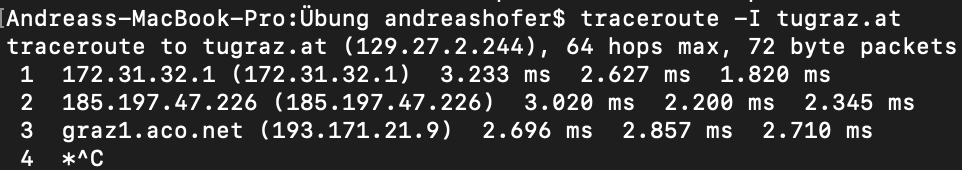
\includegraphics[scale=0.6]{Bilder/trcrt_com.png}
	\cprotect\caption{Der output von \verb|traceroute| in der command line.}
	\end{figure}
	Traceroute konnte in der command line leider nur die ersten drei Server finden, wonach alle anderen wahrscheinlich ihre IP-Adresse nicht senden wollten.
	\begin{figure}[H]
	\centering
	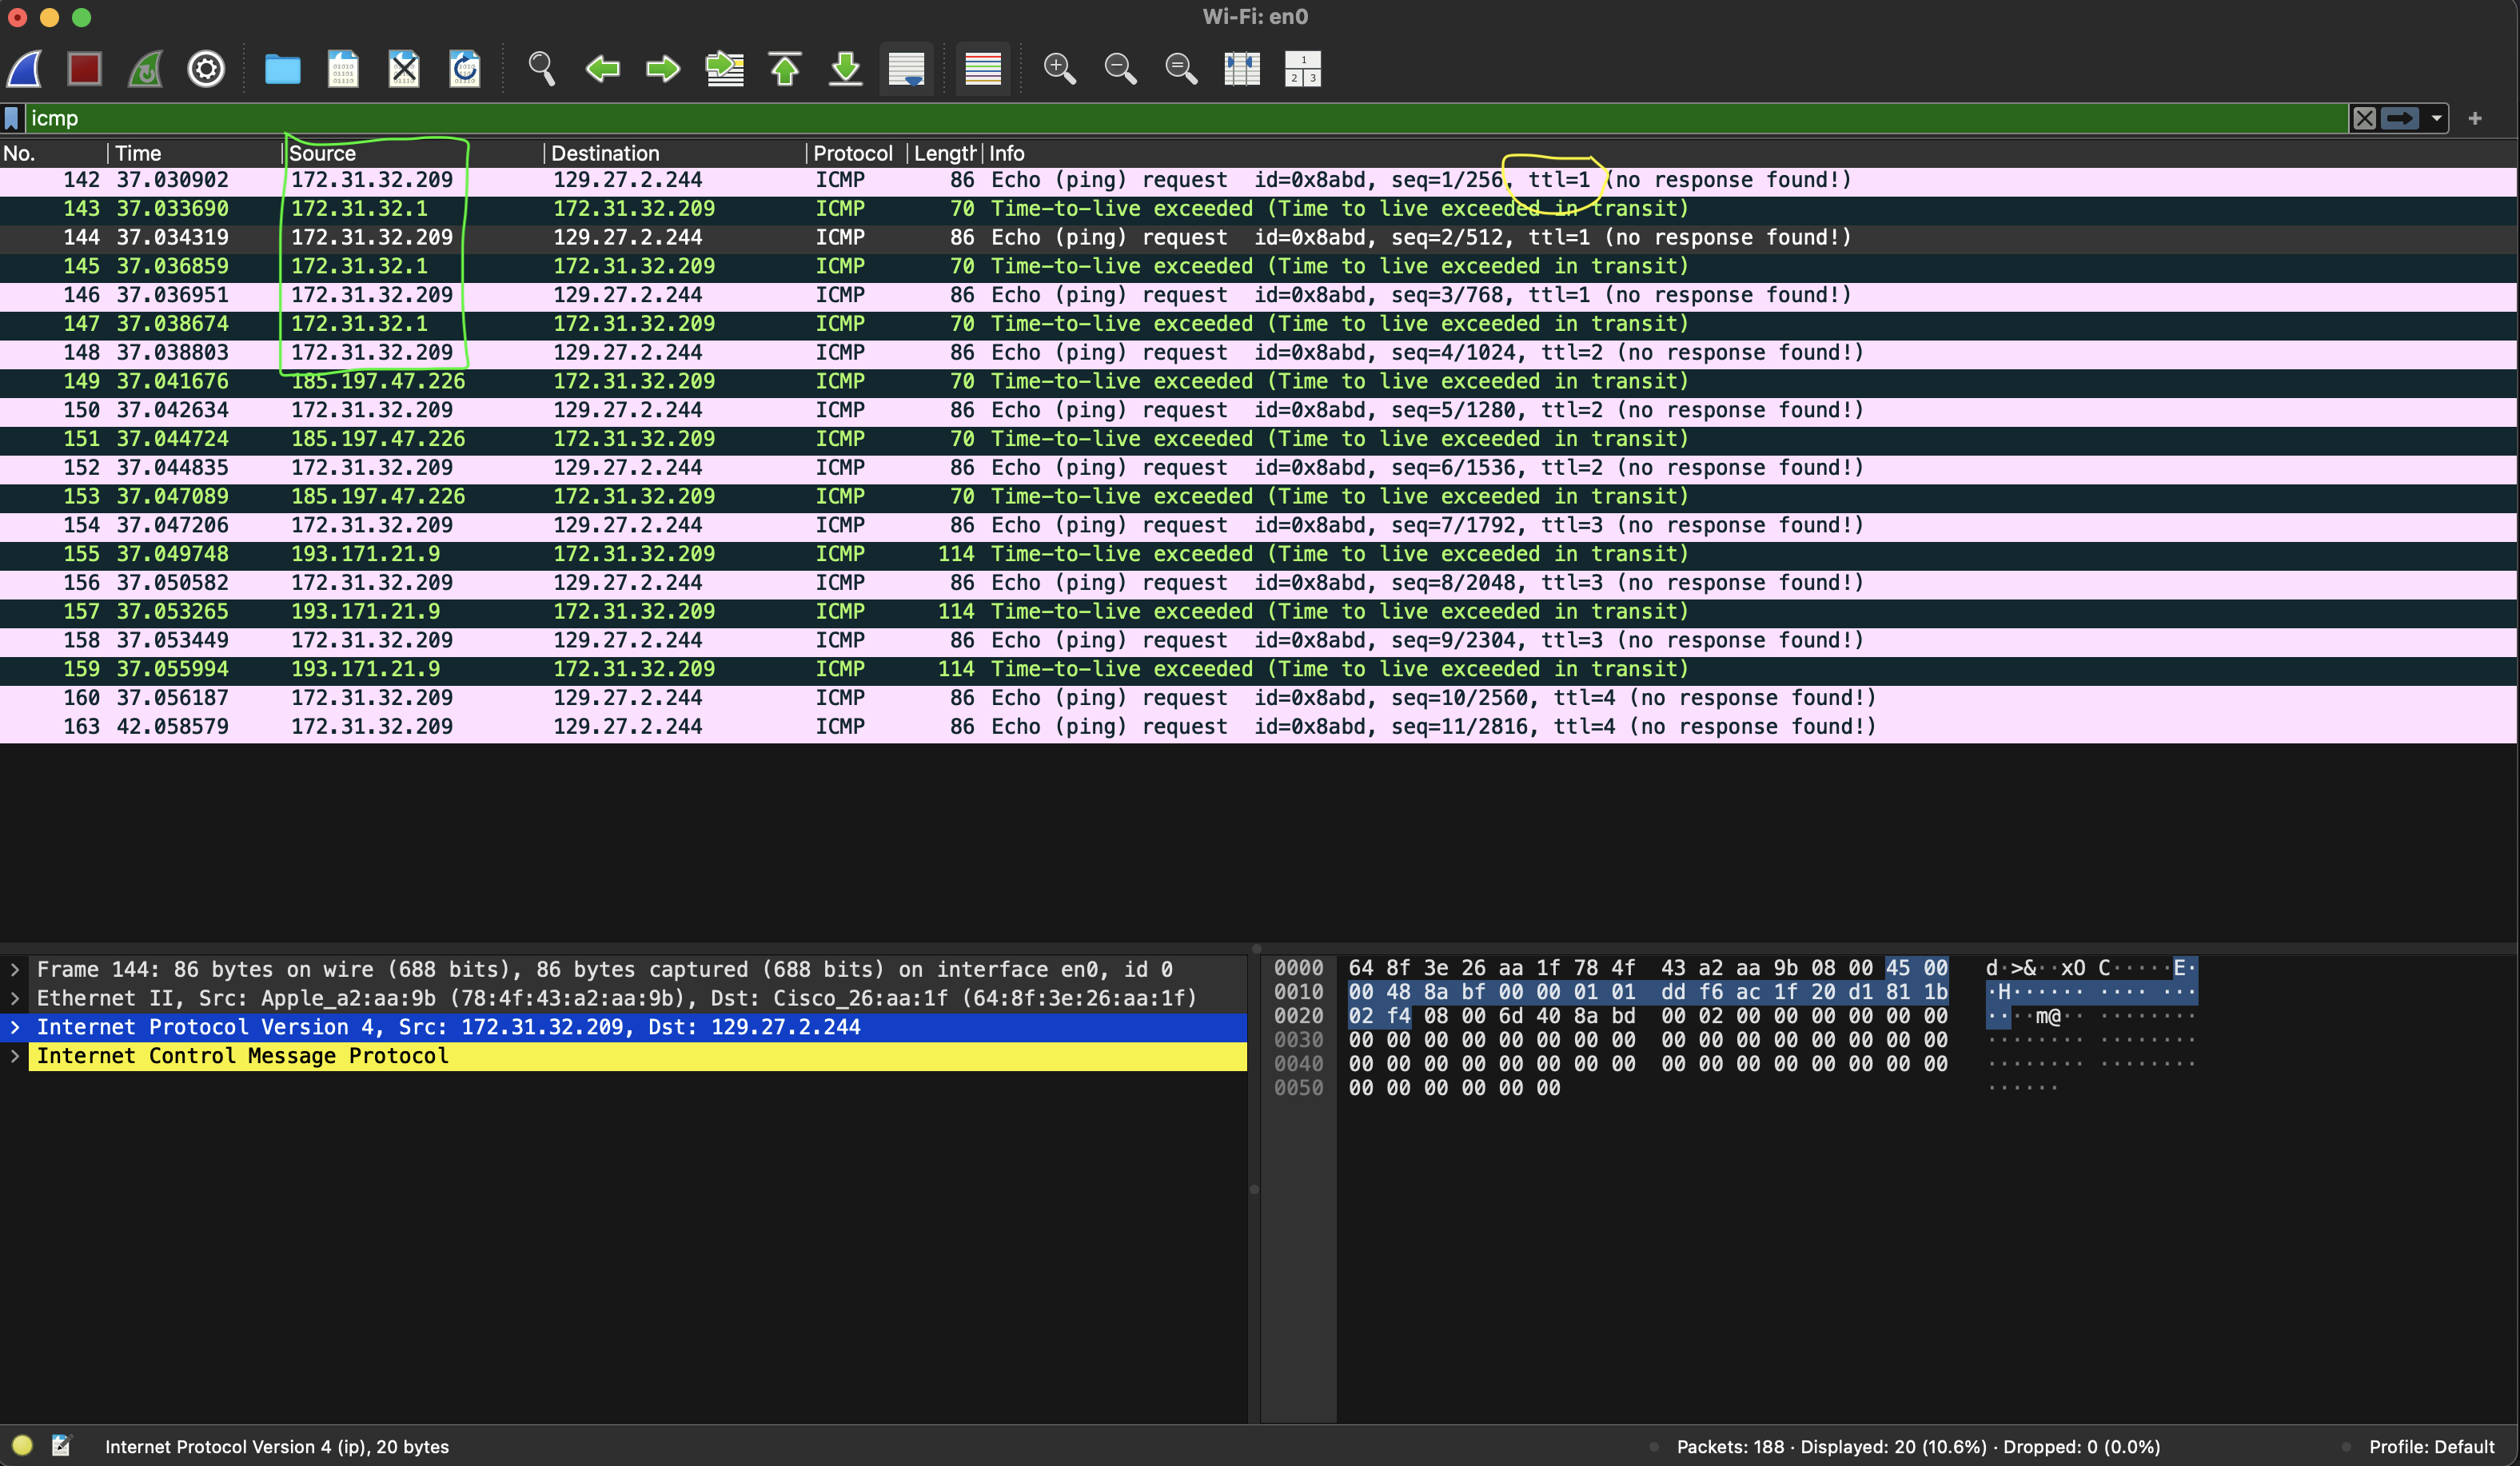
\includegraphics[scale=0.25]{Bilder/trcrt_wir.png}
	\cprotect\caption{Der output von \verb|traceroute| in Wireshark.}
	\end{figure}
	Die Wiresharkaufzeichnung des traceroute Befehls. Ich habe traceroute mit der option \verb|-I| verwendet, damit der request auch in ICMP versendet wird und so einfacher zu filtern ist. 
	\cprotect\paragraphlb{Funktionsweise von \verb|traceroute|}
	Man kann die Funktionsweise von traceroute gut sehen, ohne eines der Pakete öffnen zu müssen. Der erste request hat, in gelb, nur eine Time To Live von 1 und wird deshalb sofort verworfen und eine Antwort zurückgesendet. Das wird drei Mal wiederholt, wonach die TTL auf 2 erhöht wird. Das sollte sich theoretisch wiederholen, jedoch versendete der letzte Server (eventuell aus Sicherheitsgründen) keine Antwort. \\
	Da der erste gesendete \verb|echo| request nur eine TTL von 1 hatte, konnte dieser das lokale Netzwerk nie verlassen, wodurch er die ganze Zeit im LAN verblieb. Alle Pakete in grün, sind innerhalb des LANs da sie ja auch das selbse Subnetz als der Sender PC haben.
	
	
	
\end{document}